\subsection{Supplementary Detector Experiment Inventory}
\label{sec:supp_detector_inventory}

This supplementary section stores detector evidence that does not occupy the
main-paper comparison table. These rows are useful for reviewer transparency, but
they either expand the YOLO scale sweep, use a protocol that differs from the
main 1280-pixel comparison, or come from design-search experiments rather than
the selected detector.

\paragraph{Main/supplementary split.}
The main paper reports the selected detector, representative strong YOLO-family
and transformer baselines, and a compact related-work comparison/status table.
The supplementary material expands those results with the full YOLO-family
scale sweep, detailed related-work coverage labels, ablation details, NMS
sensitivity, heat-map analysis, and secondary dataset stress tests. This split
keeps the main paper self-contained while preserving reviewer-visible evidence
for model-scale and protocol coverage.

\begin{table*}[t]
\centering
\tiny
\setlength{\tabcolsep}{2pt}
\caption{Completed 1280-pixel detector ranking for supplementary reporting.
Rows use VisDrone2019-DET validation with seeds 42, 123, and 2026. The main
paper reports only the selected detector and representative strong baselines;
this table provides full scale coverage for reviewer inspection.}
\label{tab:supp_yolo_scale_sweep}
\begin{tabular}{rllrrrrrr}
\toprule
Rank & Group & Method & AP & AP50 & F1 & Params(M) & GFLOPs & $\Delta$AP \\
\midrule
1 & Ours & SAFR-YOLO & 0.3822 $\pm$ 0.0007 & 0.6052 $\pm$ 0.0012 & 0.6273 & 20.82 & 109.30 & +0.0045 \\
2 & YOLO large & YOLOv11l & 0.3777 $\pm$ 0.0004 & 0.5981 $\pm$ 0.0011 & 0.6248 & 25.32 & 87.30 & +0.0000 \\
3 & YOLO large & YOLOv12l & 0.3771 $\pm$ 0.0020 & 0.5958 $\pm$ 0.0025 & 0.6219 & 26.40 & 89.40 & -0.0006 \\
4 & YOLO large & YOLOv8l & 0.3765 $\pm$ 0.0003 & 0.5963 $\pm$ 0.0008 & 0.6198 & 43.64 & 165.40 & -0.0011 \\
5 & YOLO family & YOLOv9c & 0.3738 $\pm$ 0.0009 & 0.5942 $\pm$ 0.0020 & 0.6210 & 25.54 & 103.70 & -0.0039 \\
6 & YOLO large & YOLOv26l & 0.3732 $\pm$ 0.0015 & 0.5877 $\pm$ 0.0010 & 0.6136 & 26.19 & 93.20 & -0.0045 \\
7 & YOLO large & YOLOv10l & 0.3728 $\pm$ 0.0019 & 0.5890 $\pm$ 0.0020 & 0.6166 & 25.78 & 127.30 & -0.0049 \\
8 & YOLO large & YOLOv5lu & 0.3709 $\pm$ 0.0011 & 0.5897 $\pm$ 0.0017 & 0.6141 & 53.17 & 135.30 & -0.0067 \\
9 & YOLO medium & YOLOv9m & 0.3700 $\pm$ 0.0003 & 0.5910 $\pm$ 0.0012 & 0.6192 & 20.17 & 77.60 & -0.0077 \\
10 & YOLO medium & YOLOv12m & 0.3668 $\pm$ 0.0008 & 0.5851 $\pm$ 0.0029 & 0.6112 & 20.15 & 67.80 & -0.0109 \\
11 & YOLO medium & YOLOv11m & 0.3657 $\pm$ 0.0005 & 0.5846 $\pm$ 0.0012 & 0.6138 & 20.06 & 68.20 & -0.0119 \\
12 & YOLO medium & YOLOv26m & 0.3651 $\pm$ 0.0007 & 0.5801 $\pm$ 0.0005 & 0.6066 & 21.79 & 74.80 & -0.0126 \\
13 & YOLO medium & YOLOv8m & 0.3609 $\pm$ 0.0017 & 0.5771 $\pm$ 0.0012 & 0.6068 & 25.86 & 79.10 & -0.0168 \\
14 & YOLO medium & YOLOv10m & 0.3546 $\pm$ 0.0006 & 0.5674 $\pm$ 0.0016 & 0.5959 & 16.50 & 64.00 & -0.0230 \\
15 & YOLO medium & YOLOv5mu & 0.3546 $\pm$ 0.0009 & 0.5673 $\pm$ 0.0012 & 0.5988 & 25.07 & 64.40 & -0.0230 \\
16 & YOLO small & YOLOv9s & 0.3454 $\pm$ 0.0009 & 0.5573 $\pm$ 0.0011 & 0.5886 & 7.29 & 27.40 & -0.0323 \\
17 & YOLO small & YOLOv12s & 0.3338 $\pm$ 0.0015 & 0.5406 $\pm$ 0.0028 & 0.5766 & 9.26 & 21.50 & -0.0439 \\
18 & YOLO small & YOLOv8s & 0.3336 $\pm$ 0.0007 & 0.5413 $\pm$ 0.0006 & 0.5772 & 11.14 & 28.70 & -0.0440 \\
19 & YOLO small & YOLOv5su & 0.3300 $\pm$ 0.0024 & 0.5363 $\pm$ 0.0025 & 0.5718 & 9.13 & 24.10 & -0.0476 \\
20 & YOLO small & YOLOv11s & 0.3276 $\pm$ 0.0010 & 0.5304 $\pm$ 0.0018 & 0.5695 & 9.43 & 21.60 & -0.0500 \\
21 & YOLO small & YOLOv26s & 0.3254 $\pm$ 0.0008 & 0.5263 $\pm$ 0.0001 & 0.5636 & 9.96 & 22.50 & -0.0522 \\
22 & YOLO small & YOLOv10s & 0.3247 $\pm$ 0.0018 & 0.5261 $\pm$ 0.0033 & 0.5653 & 8.07 & 24.80 & -0.0530 \\
23 & Transformer & RT-DETR-L & 0.3201 $\pm$ 0.0397 & 0.5355 $\pm$ 0.0450 & 0.5773 & 32.83 & 108.00 & -0.0576 \\
24 & YOLO nano & YOLOv9t & 0.3043 $\pm$ 0.0018 & 0.4969 $\pm$ 0.0032 & 0.5379 & 2.01 & 7.90 & -0.0733 \\
25 & YOLO nano & YOLOv12n & 0.2962 $\pm$ 0.0017 & 0.4868 $\pm$ 0.0020 & 0.5309 & 2.57 & 6.50 & -0.0815 \\
26 & YOLO nano & YOLOv8n & 0.2921 $\pm$ 0.0007 & 0.4819 $\pm$ 0.0009 & 0.5242 & 3.01 & 8.20 & -0.0856 \\
27 & YOLO nano & YOLOv11n & 0.2879 $\pm$ 0.0015 & 0.4738 $\pm$ 0.0022 & 0.5197 & 2.59 & 6.50 & -0.0897 \\
28 & YOLO nano & YOLOv10n & 0.2856 $\pm$ 0.0022 & 0.4703 $\pm$ 0.0039 & 0.5160 & 2.71 & 8.40 & -0.0920 \\
29 & YOLO nano & YOLOv5nu & 0.2835 $\pm$ 0.0006 & 0.4696 $\pm$ 0.0015 & 0.5120 & 2.51 & 7.20 & -0.0942 \\
30 & YOLO nano & YOLOv26n & 0.2835 $\pm$ 0.0019 & 0.4673 $\pm$ 0.0027 & 0.5164 & 2.51 & 5.80 & -0.0942 \\
\bottomrule
\end{tabular}
\end{table*}

\paragraph{Related-work comparison inventory.}
The main paper includes a compact related-work comparison/status table so prior
detectors are visible in the detector results section. This supplementary table
keeps the detailed protocol notes. Candidate prior models must either be cited
in Sec.~2.1 or be explicitly added to the manuscript before they are treated as
paper-facing comparison rows. CSFPR-RTDETR currently has a measured external
checkpoint row and an adapter under validation. MFFSODNet and UAVDet remain
planned runnable comparisons because they have repository candidates but still
require dependency, checkpoint, and adapter audits. LEAF-YOLO-N/S are measured
external sanity checks; they should be cited explicitly if they remain in the
main related-work status table.

\begin{table*}[t]
\centering
\scriptsize
\setlength{\tabcolsep}{3pt}
\caption{Measured external related-work checks. These rows support the compact
main-paper related-work status table, but are still marked by protocol because
they use external checkpoint evaluation rather than our normalized three-seed
training protocol.}
\label{tab:supp_related_work_eval_rows}
\begin{tabular}{llrrrrrrl}
\toprule
Method & Protocol & AP & AP50 & P & R & F1 & Params(M) & Note \\
\midrule
LEAF-YOLO-S & VisDrone val, 1280 eval & 0.3080 & 0.5210 & 0.5910 & 0.5330 & 0.5605 & 4.28 & optional if cited \\
LEAF-YOLO-N & VisDrone val, 1280 eval & 0.2510 & 0.4430 & 0.5240 & 0.4610 & 0.4905 & 1.20 & optional if cited \\
CSFPR-RTDETR & VisDrone val, 1280 eval & 0.0420 & 0.1482 & 0.2805 & 0.1661 & 0.2086 & 14.09 & external checkpoint \\
\bottomrule
\end{tabular}
\end{table*}

\begin{table*}[t]
\centering
\scriptsize
\setlength{\tabcolsep}{3pt}
\caption{Related-work coverage matrix. Models discussed in Related Work are not removed from the evaluation plan; each is marked as measured, pending runnable assets, or citation-only. The live CSV version is stored in \texttt{paper/tables/related\_work\_coverage\_matrix.csv}.}
\label{tab:supp_related_work_coverage}
\begin{tabular}{llll}
\toprule
Model group & Examples & Status & Paper use \\
\midrule
Measured external eval & CSFPR-RTDETR, LEAF-YOLO-N/S & eval-only rows available; matched training adapter still under validation & Main compact status table + supplementary protocol table \\
Official repo audit & MFFSODNet, UAVDet & repository candidates identified; runnable protocol not yet staged & Coverage table and citation discussion \\
Pending compatible assets & SFFEF-YOLO, LSOD-YOLO, HF-D-FINE, DR-YOLO & code/weights/adapter not staged & Coverage table and citation discussion \\
Pending compatible assets & GCL-YOLO, SRTSOD-YOLO, YOLO11s-UAV & code/weights/adapter not staged & Coverage table and citation discussion \\
Citation-only/method motivation & LRDS-YOLO, BPD-YOLO, DG-TSOD, D2A, UFO-DETR, CFIA, DFFormer, RT-UAV-SOD & not fairly runnable today & Related-work motivation and coverage row \\
\bottomrule
\end{tabular}
\end{table*}

\paragraph{Module-search rows.}
Single-seed DCT, wavelet, CBAM, NMS, and activation-function probes are
reported as a design-search appendix, not as competing final methods. The full
ablation summary in Table~\ref{tab:supp_final_detector_ablation} keeps the
interpretable SAFR-YOLO components separate from exploratory one-seed probes,
and Fig.~\ref{fig:supp_final_detector_ablation_heatmap} visualizes their AP,
AP50, and F1 deltas relative to YOLOv11l.

\begin{table*}[t]
\centering
\scriptsize
\setlength{\tabcolsep}{3pt}
\caption{Supplementary detector ablation inventory. The first four SAFR-YOLO
component rows use the three-seed protocol. Exploratory rows are retained only
as design-search evidence and are not interpreted as final competing methods.}
\label{tab:supp_final_detector_ablation}
\begin{tabular}{lccccc}
\toprule
Ablation & Protocol & AP & AP50 & F1 & $\Delta$AP \\
\midrule
P2/P3/P4 heads & 3-seed & 0.3807 $\pm$ 0.0020 & 0.6028 $\pm$ 0.0043 & 0.6248 $\pm$ 0.0042 & +0.0030 \\
P2/P3/P4 + TinyFReLU & 3-seed & 0.3784 $\pm$ 0.0009 & 0.5987 $\pm$ 0.0018 & 0.6199 $\pm$ 0.0028 & +0.0008 \\
P2/P3/P4 + SelfAttn & 3-seed & 0.3815 $\pm$ 0.0004 & 0.6038 $\pm$ 0.0011 & 0.6256 $\pm$ 0.0025 & +0.0038 \\
P2/P3/P4 + SelfAttnFR & 3-seed & 0.3822 $\pm$ 0.0007 & 0.6052 $\pm$ 0.0012 & 0.6273 & +0.0045 \\
P2/P3/P4 + SE + TinyFReLU & 1-seed exploratory & 0.3804 $\pm$ 0.0000 & 0.6008 $\pm$ 0.0000 & 0.6243 $\pm$ 0.0000 & +0.0027 \\
P2/P3/P4 + DynFreq-P2 + TinyFReLU & 1-seed exploratory & 0.3801 $\pm$ 0.0000 & 0.6009 $\pm$ 0.0000 & 0.6213 $\pm$ 0.0000 & +0.0025 \\
P2/P3/P4 + DynFreq-small + TinyFReLU & 1-seed exploratory & 0.3815 $\pm$ 0.0000 & 0.6034 $\pm$ 0.0000 & 0.6233 $\pm$ 0.0000 & +0.0038 \\
\bottomrule
\end{tabular}

\end{table*}

\begin{figure*}[t]
    \centering
    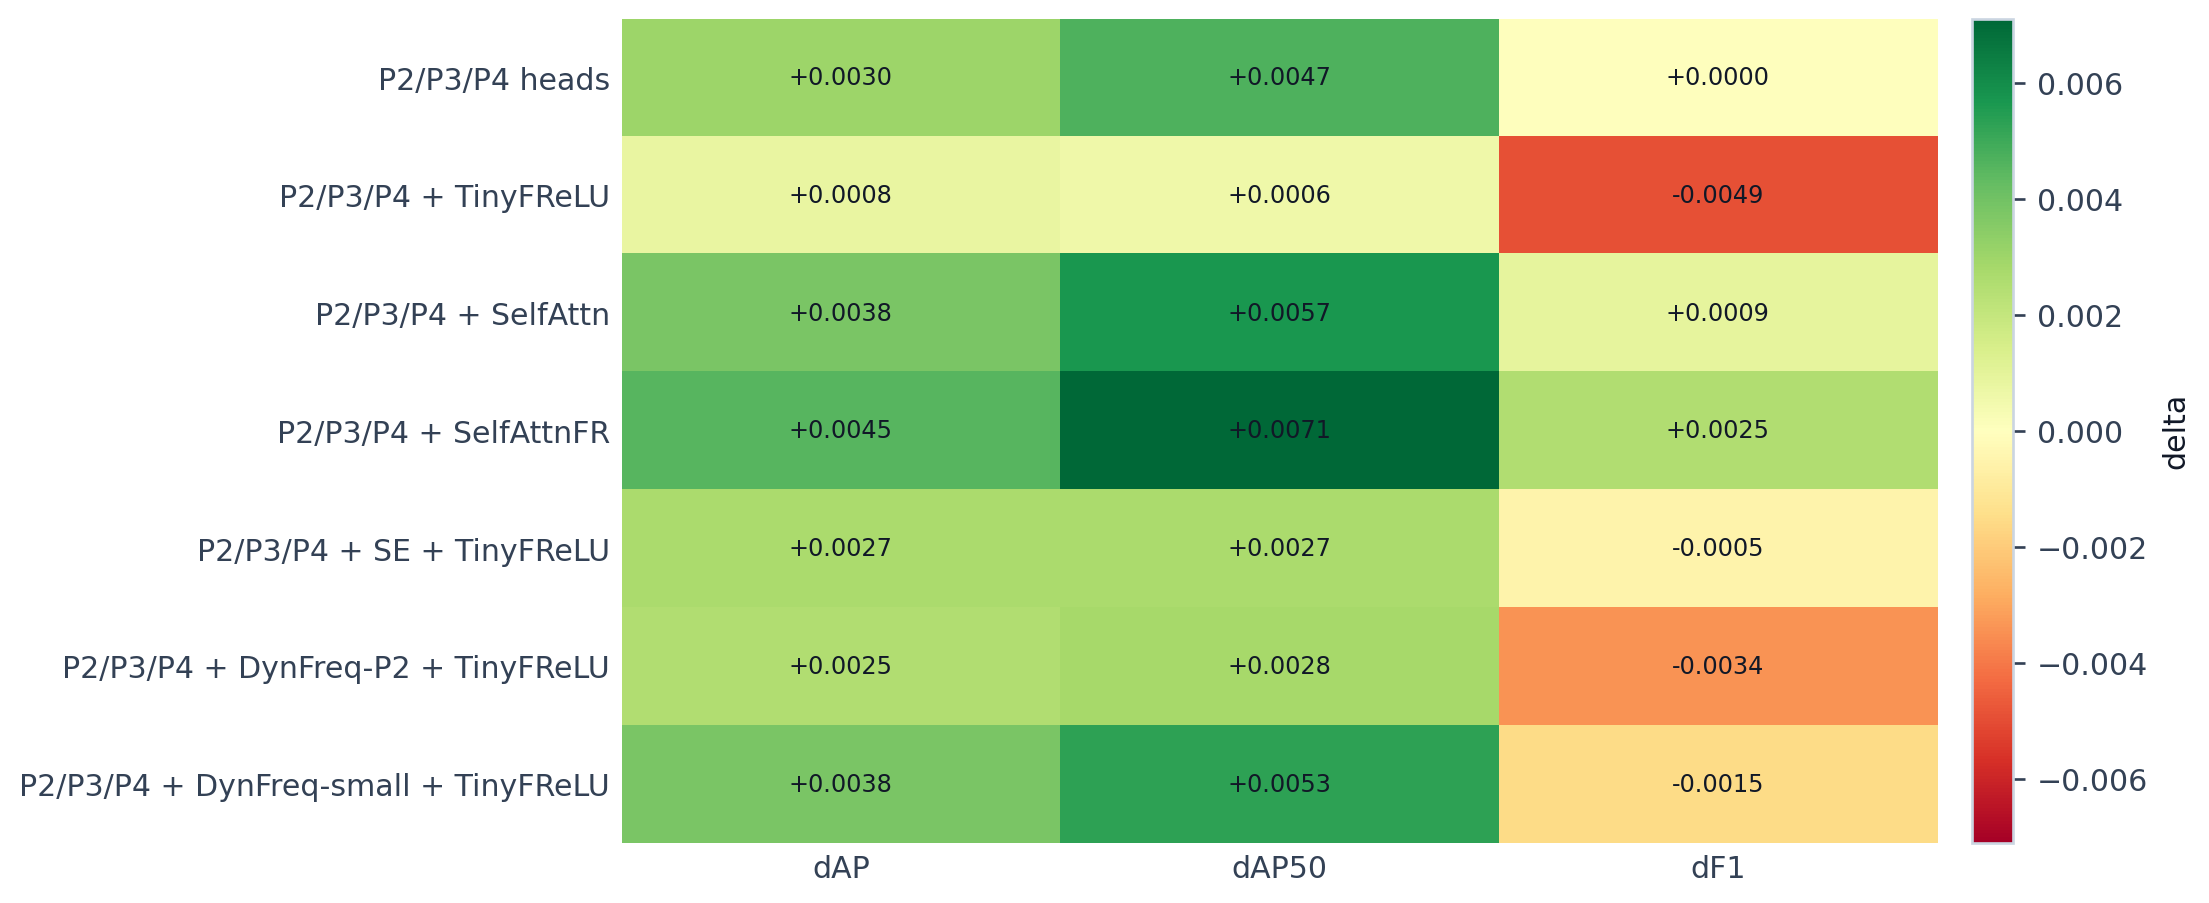
\includegraphics[width=0.78\textwidth]{figures/results/paper_fig10_final_ablation_metric_heatmap}
    \caption{Supplementary ablation heatmap showing AP, AP50, and F1 deltas
    relative to YOLOv11l. Green cells indicate improvements over the baseline,
    while red cells indicate regressions.}
    \label{fig:supp_final_detector_ablation_heatmap}
\end{figure*}

\paragraph{Planned qualitative and explainability figures.}
The following supplementary slots are reserved for the final detector checkpoint
and Grad-CAM output. These figures are not headline claims until generated from
the final checkpoint.
\begin{itemize}
    \item Supp. Fig.~S4: side-by-side Grad-CAM or detector heat maps for
    YOLOv11l and SAFR-YOLO on crowded UAV crops.
    \item Supp. Fig.~S5: qualitative detection examples grouped by small
    vehicles, pedestrians, dense adjacent objects, and water/road clutter.
    \item Supp. Fig.~S6: failure cases, including missed tiny objects,
    false positives from shadows/reflections, and overlapping-box errors.
    \item Supp. Fig.~S7: input-resolution stress test, reported only after the
    final 1280 detector claim is fixed.
\end{itemize}

\paragraph{Post-processing sensitivity.}
Overlap-aware NMS is reported here unless a complete three-seed
confirmation is added to the main detector protocol. The current NMS snapshot is
useful because it shows that adjacent-object post-processing can improve AP and
AP50 on a fixed checkpoint, but the paper labels it as an eval-only
robustness analysis.

\paragraph{TinyPerson supplementary stress test.}
TinyPerson is reported as a detector-only supplementary stress test after
the final VisDrone detector is fixed. The planned compact table contains
YOLOv11l, the final SAFR-YOLO detector, and one compact architecture-only
variant at 640-pixel input. Related-work TinyPerson rows are added only
for models that are either cited in the manuscript or explicitly added to the
Related Work section with a matching bibliography entry.
